\documentclass[a4paper,12pt]{article}
\usepackage{graphicx}
\usepackage{float}
\usepackage[T1]{fontenc}
\usepackage{hyperref}
\graphicspath{ {./images/} }
\pagenumbering{gobble}
\begin{document}

\author{Miłosz Wojciechowski}
\title{Telemetry extractor manual}
\date{\today\\ v0.3}


\maketitle
\pagebreak
\pagenumbering{arabic}
\renewcommand{\labelenumii}{\arabic{enumi}.\arabic{enumii}}

\begin{enumerate}
	\item Record a video with your GoPro camera (traditional video in HERO or 360 mode, Time Lapse in traditional or 360 mode). Make sure that you have turned on GPS function:
\begin{figure}[H]
	\centering
	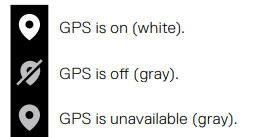
\includegraphics{GoPro_manual_fragment}
	\caption{GoPro Max manual fragment.}
\end{figure}
	If GPS is off, swipe down to access the Dashboard and Preferences. Click on the Preferences, find option Regional and there turn the GPS On.\\
	\item Download repositories: \href{https://github.com/JuanIrache/gopro-telemetry}{gopro-telemetry} and \href{https://github.com/JuanIrache/gpmf-extract}{gpmf-extract} and unpack them in GoPro-Telemetry-Extractor directory.
	\item Install Node.js from \url{https://nodejs.org/en} using recommended download.
	\begin{figure}[H]
		\centering
		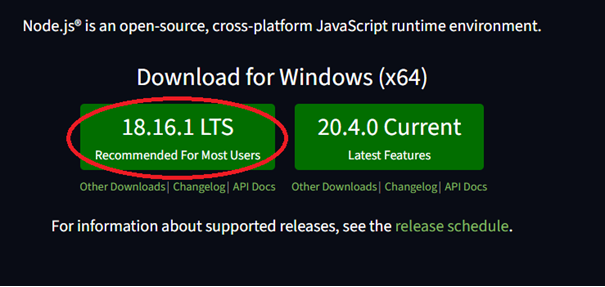
\includegraphics{nodejs_install}
		\caption{Nodejs website fragment.}
	\end{figure}
	To check if installed correctly simply open Command Prompt by typing “cmd” in the Start Menu and write “node”, if everything was done properly version of node should appear.
	\begin{figure}[H]
		\centering
		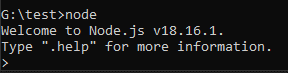
\includegraphics{node_confirmation}
		\caption{Command Prompt fragment confirming proper installation of Nodejs.}
	\end{figure}

	\item Extract .LRV file into directory where repository was downloaded, steps explaining how to do it are shown below:
	\begin{enumerate}
		\item File structure of GoPro Max videos:
		
		GoPro Max creates 3 types of files during recording, in 360 mode we get:
		\begin{itemize}
			\item .360 file (main video file)
			\item .THM file (thumbnail file)
			\item .LRV file (low-res video file)\\
		\end{itemize}
		In HERO mode (traditional video in 1080p or 1440p) we get:
		\begin{itemize}
			\item .MP4 file (main video file)
			\item .THM file (thumbnail file)
			\item .LRV file (low-res video file)\\
		\end{itemize}
		These files always appear after recording a classical video or a Time Lapse.\\ 
		
		\item Recordings location:
		
		To reach it, plug your GoPro Max camera to a computer using USB-c to USB cable. Now find your connected GoPro camera and navigate through directories:\\
		
		$\textit{GoPro MAX > GoPro MTP Client Disk Volume > DCIM > 100GOPRO}$	\\
		
		Final path should look like this:
		
		\textit{GoPro MAX/GoPro MTP Client Disk Volume/DCIM/100GOPRO}	
		\begin{figure}[H]
			\centering
			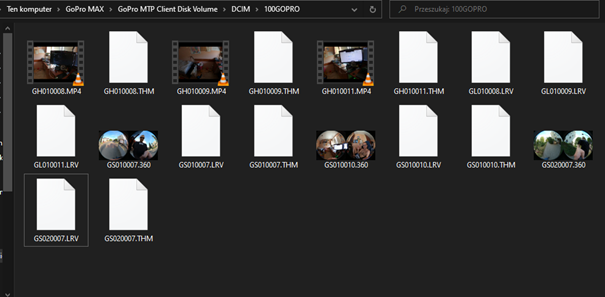
\includegraphics{recording_location}
			\caption{Video files location.}
		\end{figure}
		\hfill
		\item Choose video which you want to extract telemetry data from and copy it to a folder where repository was downloaded so a video file and extractor.js are in the same directory:\\
		
		360 videos’ names and their LRV versions start with GS e.g. GS020007.360, GS020007.LRV.\\
		
		Regular videos’ and their LRV versions’ names start with GH for the former and with GL for the latter e.g. GH010008.MP4, GL010008.LRV. \\
		While only extracting telemetry i suggest using LRV file since it will work much faster.
	\end{enumerate}
	\item Open Command Prompt by typing “cmd” in the Start Menu and navigate to extractor.js location.
	\item When in proper directory run the program by writing “node extractor.js <your video file> e.g. 'node extractor.js GS020007.LRV'. Telemetry .csv file will appear in the same location as extractor.js file.
	\pagebreak
	\item To show trajectory on a map open \\ 
	\url{https://mygeodata.cloud/converter/csv-to-gps}, load received earlier .csv file and click “Show in a Map”.
	\begin{figure}[H]
		\centering
		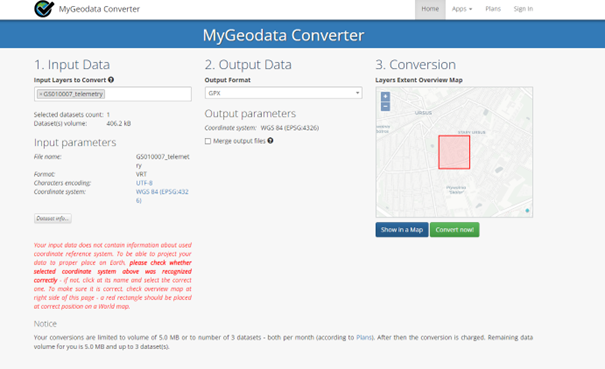
\includegraphics{Map_page}
		\caption{MyGeodata website to convert a csv file to GPS and view it on a map.}
	\end{figure}
\end{enumerate}
 
\end{document}